\chapter
 [Compiling Qoala programs]
 {Compiling Qoala programs}
\label{chp:compiler}


\begin{abstract}
In this chapter, we deal with the question of compiling Qoala programs.
Compilation involves two elements: translation from a higher-level program representation (like a human-friendly programming language) to 
a lower-level representation (such as assembly instructions), and optimization of the program with respect to certain metrics.
Optimization metrics include offline ones such as instruction count and memory usage, and online ones such as success probability.
Many existing compilation strategies, of both classical and quantum computing, can be re-used.
However, unique challenges are presented by the nature of quantum network programs.
In this chapter, we outline these challenges and present an architecture of a compiler that address these challenges.
We then report on a preliminary implementation and point to future evaluation and extension ideas.
\end{abstract}

\subsection{Introduction}
As described in the introduction and in previous chapters, quantum network applications consist of programs that are executed on the nodes of the network.
For these programs to be executable, they must be in a specific format.
In \cref{chp:qoala} we presented the Qoala execution environment, being an improvement over the QNodeOS (\cref{chp:qnodeos}) runtime.
Qoala requires the programs to be in a specific format, including classical and quantum instructions, and where some parts are represented using the NetQASM assembly language (\cref{chp:netqasm}).

Although programmers could express their program logic directly in the Qoala format, this is not practical for several reasons.
First, since the format is low-level, it is quite verbose.
This is a similar issue as with classical assembly (or other lower-level languages): although possible, it is often very impracticle to write complete programs in assembly itself.
Second, the low-level format can be quite far from the high-level program logic.
Someone who wants to implement a certain quantum network program typically only cares about the overall (high-level) behavior of the program.
For example, they might simply want to express that the program should create entangled states repeatedly, and then measure all created qubits.
Having to deal with low-level details about how express looping behavior, which (quantum) memory and how much to allocate, and how to integerate the classical and quantum code
is in most cases not something a programmer wants to deal with. 
Third, the Qoala program format allows hardware-specific details, such as hardware-specific quantum instructions (using NetQASM flavors, see \cref{chp:netqasm}).
Although not required to add these details by the programmer, if one wants to make use of these details to improve execution (e.g. increasing success probability), the programmer should have knowledge about the hardware.
Ideally, the programmer should not have to write different versions of a program, one for each hardware platform that the program is intended to run upon.

The Qoala program format was indeed not intended to be used by programmers directly.
\reminder{focus on programmers: can we say something about practical feedback, i.e. actual users of our tools?}
Instead, it was envisioned that a programmer would express program logic in a high-level language, such as Python, and that a compiler would transform this into a Qoala program.
Allowing expression in such a higher-level language takes away the aforementioned issues.

Program compilation is a well-studied topic in both classical and quantum computing and is a vital tool in everyday practical software development.
Many existing ideas and strategies can be re-used for compiling quantum network applications.
However, quantum network applications present unique challenges that need to be solved by a compiler.

First, there is a distinction to be made between compiling applications and programs.
Compiling the whole (multi-node) application is not something we consider here.
Indeed we treat programs (single-node) to be independent and having an independent compiler.
Figure \todo{Schematic of application compilation vs program compilation} illustrates this.
Compiling a whole application would be similar to compilation for distrbuted quantum computing.
Second, programs are inherently hybrid in nature: they contain both classical and quantum code.
\todo{Why difficult?}
Third, optimization is not clear.
Runtime performance not only depends on the compilation, but also on scheduling.

- general
  - program-application distinction
  - difference with distrbuted qc
  - classical-quantum interactivity
  - success metric also depends on scheduling

- qoala-specifc
  - netqasm flavors
  - deadlines
  - using EHI

\todo{Difference with QNodeOS compiler}

% A quantum internet, consisting of programmable quantum computers that can communicate with each other, enables the execution of applications that are not possible in a classical internet nor on a single quantum computer.
% Such applications leverage the unique properties of quantum entanglement to achieve their goals.
% Quantum internet applications consist of a set of programs, each executed by a node in the network.
% These programs interact with each other by sending classical messages and by using entangled quantum states.
% Examples of applications include Quantum Key Distribution (QKD), Blind Quantum Computation (BQC), secret sharing protocols, and agreement protocols.

% Realizing such applications requires certain key ingredients.
% First, a description of the programs constituting the application must be given: what operations must each of the nodes do and when?
% Second, a runtime environment on each of the nodes which can handle program descriptions and can execute the operations described in them.
% Furthermore, the quality of application execution depends on the operations applied, the timing of these operations, and the hardware characteristics of the nodes.
% Since quantum states decohere (degrade in quality) over time, controlling the timing of operations is important to achieve performant execution.

% A runtime environment that can execute quantum internet programs exists: Qoala.
% Qoala also allows scheduling of program components, enabling optimization of execution.
% However, Qoala takes as input program descriptions that are low-level, meaning that they do not allow complex abstractions.
% This design has been made on purpose, such that the Qoala specification is relatively simple, and such that an implementation can be relatively simple.

% In order to make it easier for programmers to express their application logic, however, a more sophisticated program representation is needed.
% Such a representation enables programmers to focus on the logic, and not have to deal with low-level implementation and optimization details.
% If programmers represent their application logic in a high-level representation, necessarily a translation step must be performed from this representation to the lower-level Qoala representation.

% Since applications consist of multiple cooperating programs, some kind of coordination is required.
% The order of external operations in a program (message-passing and entanglement generation) must match with external operations in other programs.
% An application protocol description is needed such that programmers know in which order they have to put their operations.

\subsection{Design considerations}
Let us recap what our objectives are.

\textbf{Translation from high-level to Qoala.}
First we must decide on a high-level format.
Questions like memory-based, value-based?
We may also want to allow multiple (existing) high-level formats.

Then, translation itself needs to be done. 
A common strategy in compilers is to use one or more intermediate representations.

\textbf{Optimization.}
Optimization must be trackable \todo{*must* be?} by metrics.
There are different metrics.
In quantum computing, there is circuit depth, circuit width.
In general there is also compilation time.

For quantum network programs there is also success probability.


\subsection{Objectives}
- Execute quantum internet programs efficiently in terms of application success probability and success rate
- Improve accessibility by enabling programming using high-level concepts and tools
- Provide a framework for coordinating programs in a multi-node application

Efficient execution requires timing and scheduling control over the programs, because of *time-sensitivity* and because of the *multiprocessing environment* of nodes.
Also, programs are *hybrid in nature*.
Therefore, Qoala is used as the target runtime.
In the Qoala execution framework, *capability negotiation* is required; this leads to the need of some external protocol description.


Ingredients minimally needed:
- a high-level program source code language suitable for programmers
- a protocol specification format for coordinating programs in a multi-node application
  - includes retries?
- valid (for target) translation to Qoala machine code

Additional ingredients:
- fidelity and timing constraints in program and protocol
- noise-aware optimization


Choices and assumptions:
- We want to re-use existing infrastructure and not re-invent the wheel. This means we can make use of or take inspiration from:
  - classical compilers with traditional translation and optimization strategies
  - quantum compilers with circuit mapping and gate optimization techniques
- We will use Intermediate Representations (IRs) to bridge the gap between the source code and machine code.
- The front-end language is not a primary concern; we want to leave design and implementations open.

\subsection{General considerations}
It's only **live quantum memory** that's time-sensitive.
The Qoala runtime provides a way to schedule and prioritize program parts such that quantum decoherence can be minimized.
To take advantage of this, quantum code, possibly interspersed with classical code, should be executed as Qoala programs.
However, it is not needed to write a whole program, including parts with purely classical code, in Qoala.


\subsection{Related work}
Catalyst
TODO

\subsection{High-level choices}
\begin{itemize}
\item Why python
  Since it first launch, python was positioned as a programming language that allows the programmer to quickly develop
  solutions with less lines of code. Lowering the usual barriers from other programming language is what allowed python
  to gain popularity among the scientific community.
  The Qoala platform goes in this line by allowing the scientific community to write quantum internet programs in a
  language that is easy to use, that is easy to understand, and that is known by the scientific community.
\item Why MLIR
  MLIR is a modular and extensive compiler infrastructure that allows extending the LLVM infrastructure, easing the
  developing of domain-specific representations and allowing reusing other pieces of the LLVM compiler infrastructure.
  By allowing the definiton of \textit{dialects}, MLIR allows extending the intermediate representations of the clang compiler
  pipeline, enabling the conversion of programs between different dialects, and also alowing the re-usage of the
  optimizations and analysis implemented in other dialects.
  All these feature make MLIR a perfect candidate for creating the compiiler for hybrid quantum internet programs.
\item Why iqoala as output
\item Why protocol description
\end{itemize}
    

\subsection{Optimizations}
We consider the following optimizations:
\begin{itemize}
\item qubit mapping optimization (already exists)
\item gate-level optimization (already exists)
\item classical-quantum division (limit host-qnodeos communication and limit qubit lifetimes)
\item inserting deadlines to try and meeting timing and fidelity constraints
\end{itemize}


\subsection{Architecture}


\begin{itemize}
\item High-level MLIR Dialect (QoalaHIR)
    \begin{itemize}
        \item Hybrid classical-quantum
        \item No memory allocation
        \item Timing and fidelity annotations
        \item Entanglement as abstract operation
    \end{itemize}
\item Low-level MLIR Dialect (QoalaLIR)
    \begin{itemize}
        \item Explicit split between classical and quantum code
        \item Memory allocation
        \item Timing and fidelity annotations
        \item Entanglement as abstract operation
    \end{itemize}
\item Translation passes:
    \begin{itemize}
        \item HIR -> LIR
        \item Codegen LIR -> QoalaHost instructions
        \item Codegen LIR -> NetQASM
    \end{itemize}
\item Optimization passes:
    \begin{itemize}
        \item Memory mapping on quantum LIR
        \item Find best split between cLIR and qLIR when translating HIR -> LIR (can be pass on HIR before translation)
        \item Convert fidelity constraints into timing constraints
        \item Extract constraints from protocol description into HIR annotations
    \end{itemize}
\end{itemize}

\subsection{Related work}
\begin{itemize}
    \item Hybrid language: does not yet exist for networking
    \item Protocol description language: (timed) session types
    \item compiler to Qoala does not yet exist
    \item fidelity and timing constraints don't really exist
    \item noise-aware optimization for circuits exists, not for interactive hybrid programs
\end{itemize}


\subsection{Compilers}
Traditionally, a compiler has three purposes:
(1) translation of a high-level program representation to a low-level executable one,
(2) error-detection in the program source code,
(3) optimization of the program with respect to the runtime environment including the hardware.

\textbf{Translation}. Allowing a programmer to write application logic in a high-level language improves the accessibility: it relieves the programmer of the burden of thinking about low-level details, and makes it easier to express complex logic. However, in the end, hardware must execute low-level code and a translation step is required. Such translation must maintain the intended behavior of the program (correctness).

\textbf{Error detection}. A compiler checks whether the program source code is valid and throws an error if it is not.

\textbf{Optimization}. A compiler tries to optimize the final executable in various way. (1) It might try to minimize the size of the final executable. (2) It might try to produce an executable such that the expected runtime performance is optimized.

\section{Qoala}

\subsection{Considerations}

\textit{Modes of compilation}. Quantum internet programs run in the context of a multi-node application.
This means that programs must coordinate in some fashion in order to produce meaningful behavior.
For example, they must follow a certain protocol.
We distinguish two Modes of Compilation (MoC):
\begin{itemize}
    \item Protocol-informed compilation: a pre-defined protocol exists describing at least the order of interactive steps that the nodes must execute. A compiler may take advantage of such a protocol description.
    \item Standard compilation: there is no pre-defined description of a protocol, and a compiler cannot take advantage of such knowledge.
\end{itemize}

\textit{Steps needed before execution}.
Demand registration to network controller. To make an informed demand, a protocol description is needed such that nodes can synchronize their behavior and agree about timings, iterations, and retry mechanisms. Therefore, it makes sense to already have a protocol description at compile-time. This can also e.g. be something that is advertised as a service by some quantum server.

\textit{Protocol description}.
\begin{itemize}
    \item Must contain: order of interactive steps
    \item May contain: timing constraints
    \item May contain: fidelity of states
\end{itemize}

\textit{Protocol-uninformed compilation}.
\begin{itemize}
\item Inputs: program code (may contain fidelity/timing constraints), EHI
\item Compilation:
    \begin{itemize}
        \item General correctness checking
        \item Translation to valid Qoala
        \item Optimization:
            \begin{itemize}
                \item General (gate optimization etc.)
                \item Insert hints to try and meet fidelity/timing constraints from program
                \item Cannot re-order external operations
        \end{itemize}
    \end{itemize}
\item Capability negotiation:
    \begin{itemize}
        \item Potentially refer to protocol description and claim compatibility
        \item Establish demand, number of instances, inputs, deadlines
        \item This is a "parallel" WIP by other people from the team. We need to stay aligned with them.
    \end{itemize}
\item Inputs: program code (may contain fidelity/timing constraints), EHI
\end{itemize}

\textit{Protocol-informed compilation}.
\begin{itemize}
    \item Inputs: program code (may contain constraints), EHI, protocol description (may contain constraints)
    \item Compilation:
    \begin{itemize}
        \item General correctness checking
        \item Adherence to protocol checking
        \item Translation to valid Qoala
        \item Optimization:
        \begin{itemize}
            \item General (gate optimization etc.)
            \item Insert hints to try and meet fidelity/timing constraints from program
            \item Insert hints to try and meet fidelity/timing constraints from protocol
            \item Cannot re-order external operations
        \end{itemize}
    \end{itemize}
    \item Capability negotiation: Establish demand, number of instances, inputs, deadlines
\end{itemize}

\textit{Capability negotiation}. Needed since demand registration is needed. Must be after compilation such that same executable can be re-used in multiple contexts. Uses input from users (that are about to run the application) and uses hints from the compiler (put into the executables). Also uses input from network controller (like current estimates of rate, fidelity).


\textit{Translation to valid Qoala}. Need to adhere to EHI, which includes flavour and topology.



\subsection{High-level language}
Needs to allow classical and quantum code, interleaved.

May allow fidelity constraints and timing constraints.

\begin{itemize}
    \item Fidelity constraints in high-level program code. Needed to get success probability (especially since other programs may run in parallel; it's a way to define implicit priority)
    \item Timing constraints in high-level program code. Why needed?
\end{itemize}


\subsection{Protocol description}
\begin{itemize}
    \item Fidelity constraints in protocol. Needed since otherwise protocol may not be valid anymore (e.g. BQC is not secure anymore if EPRs are below certain fidelity). Indirectly informs (through compilation and then capability negotiation) the demand registration.
    \item Timing constraints in high-level program code. Why needed?
\end{itemize}



\section{High-level design}

\subsection{Overview}
The figure below presents the general architecture of the Qoala compiler:

\begin{figure*}[ht]
    \centering
    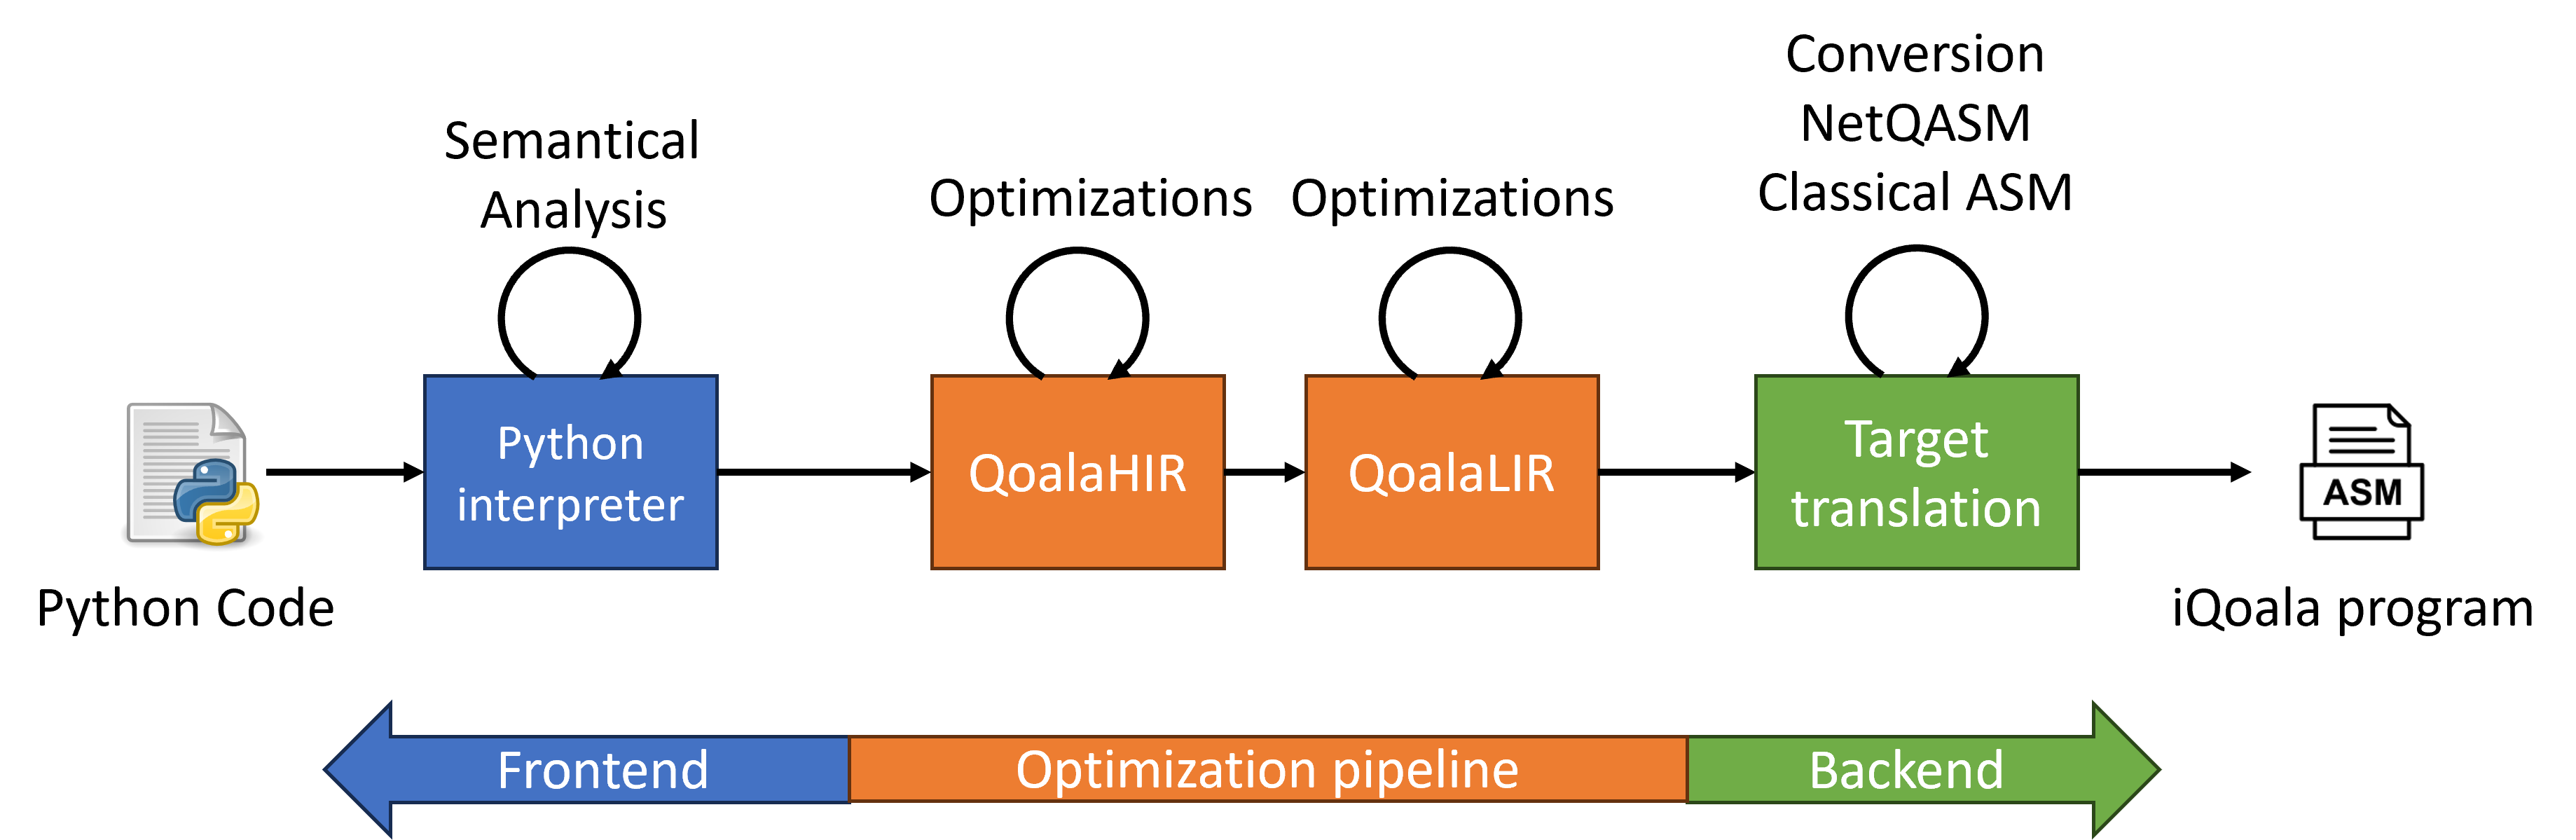
\includegraphics[scale=1.0]{figures/compiler/compiler-arch.png}
    \caption{Qoala compiler stages}
    \label{fig:qoala_compiler_stages}
\end{figure*}


The core steps in the Qoala compilation process are:

\begin{itemize}
\item Programmer writes source code in Python using the Qoala Python SDK.
\item The Python SDK itself provides a `compile` function that executes the source code
  which produces a `.mlir` file containing the program code in QoalaHIR format.
\item This Python SDK implements \textit{some} functionality present in the "frontend" of a classical
  compiler, for example, a semantical analysis to check the validity of the classical and
  quantum operations specified in the program 
\item A separate `opt`-like tool (built using LLVM/MLIR) takes the `.mlir` as input and produces
  (after several applying passes) a `.iqoala` file.
\item The `.iqoala` file can then be executed by a Qoala runtime.
\end{itemize}


\subsection{Context of Qoala programs}
A Qoala program spans across the whole lifetime of qubits.
Multiple Qoala programs may be run separately, but they cannot share quantum memory (qubits).
This means that the physical Qubits used by one program *cannot be used* by another one, not
even when preempting tasks.

To correctly allocate the quantum resources and avoid *statically* tying the program to use
certain physical qubit, the binary relies on the Quantum Resources Management Unit (QResMU) to map
the physical quantum resources to the virtual values used by the program instance.


\subsection{Python SDK}
The Python SDK is a library containing classes and methods that allow:
- expressing quantum internet program logic, and
- producing a QoalaHIR representation of the source code

The general should look like this:

\begin{pycode}
class MyProgram(QoalaProgram):
    def main(self, ctx: QoalaContext):
        q = ctx.new_qubit()
        e = ctx.entangle_keep("Bob")
        ctx.cnot(q, e)
        m = ctx.measure(q)
        ctx.add_return(m)

program = MyProgram()
mlir = program.compile()  # `compile` is defined in `QoalaProgram`
with open("program.mlir", "w") as f:
    f.write(mlir.text())
\end{pycode}

The Python SDK acts as the "frontend" of the qoala compiler. In this sense,
the output of the Python SDK is a `.mlir` file in the QoalaHIR dialect.
By using Python as a the high-level language of the programs, we can take advantage
of the python interpreter to perform the parsing of the code and an initial
syntactical analysis.
To complete the frontend analysis, the Qoala libraries could also embed a
semantical analysis to check the correctness of the applied quantum operations.
As mentioned before, the main goal of this Python SDK (frontend) will be to
create a High Level representation of the program, using the QoalaHLIR
language, which will be the main input of the optimization pipeline int he next stages.


\subsection{MLIR-based optimizer pipeline}
The Qoala compiler also defines an optimization pipeline that analyses and
transforms the code to improve its performance and prepare it for the final
translation in the iQoala format.

To this end, the optimization pipeline makes use of the MLIR framework to
define intermediate representations as *dialects*. Later, the optimization
tools can apply *passes* on the intances of the program expressed using the
MLIR dialects.


\subsection{Representations and dialects}
The Qoala compiler uses three intermediate representations (IRs) when in the "MLIR-phase".
These are the High-level Intermediate Representation (HIR), Mid-level Intermediate Representation (MIR), and the Low-level Intermediate Representation (LIR).
Each IR is associated with a particular set of MLIR dialects.
The Qoala compiler uses four custom MLIR dialects, called `QNet`, `QMem`, `QoalaHost`, and `Netqasm`, explained in more detail below.

\begin{itemize}
\item HIR (High-level): A higher-level IR, where operations are closely related
  to the python source.
  Quantum operations are represented using the `QNet` dialect, which consume and produce quantum *values*.
  Programs in the HIR format use the following dialects: `QNet`, `arith`, `scf`, `affine`, `async`, `tensor`.
\item MIR (Mid-level): A mid level IR, similar to HIR but with explicit memory locations, using the `QMem` dialect instead of `QNet`.
\item LIR (Low-level): A lower level IR, where operations are closer to the
  classical and quantum assembly instructions.
  Quantum operations are represented using the `Netqasm` dialect, which take quantum *registers* ("quantum memory pointers") as operands
  and have side-effects on the quantum value stored in the registers.
  Programs in the LIR format use the following dialects: `QoalaHost`, `Netqasm`, `arith`, `scf`, `affine`, `async`.
\end{itemize}

Tranforming from HIR to LIR hence involves lowering QNet operations to QoalaHost and Netqasm operations.
On top of that, both HIR and LIR have additional constraints about the structure of code in that representation which need to be respected.


\subsubsection{General optimization pipeline}
The MLIR optimization pipeline applies the folliwng operations:
\begin{itemize}
\item apply optimzation passes on the QoalaHIR code
\item transform QoalaHIR to QoalaLIR
\item apply optimzation passes on the QoalaLIR code
\item generate `.iqoala` code from QoalaLIR
\end{itemize}

This optimization pipeline introduce modifications in different levels of the process:
\begin{itemize}
\item At HIR level: operations can be re-order, respecting the restrictions specified
  [in the HIR specification document](dialects/HIR.md).
\item Conversion from HIT to LIR: High-level qubit allocations instructions are exploded
  into the lower-level qubit allocation operations, which includes allocation,
  initialization and value writing/reading.
\item At LIR level: operations belonging to the same local quantum functions are grouped
  into functions ("functionize") to aid the scheduling at runtime.
\end{itemize}


\subsubsection{Memory Alloc (i.e. Qbits allocation)}
- Entanglement move to memory qubti??
- Use/keep of subroutines in iqoala ??

Idea: try to stitch together separate functions/subroutines to get one circuit and apply standard circuit optimizations on it.
Does not really work: in general programs can have many different circuits at runtime depending on control-flow.

Maybe: first functionize, then check qptrs that are passed into/out of function calls? Then try to map these pointers to as few qubit IDs as possible.

??? Legalize to specific Unit Module. E.g. for NV with 2 qubits, a cphase gate must be between a comm qubit and a mem qubit. So, values used in cphase operation must come from comm pointer and mem pointer respectively. 
- Do a normal pass? or
- Bake constraint into dialect? (but then: dialect needed for each different UM)

\subsubsection{Pass: memory alloc by assigning constants?}
Maybe first use QubitPointers. Then with an optional pass: assign constant values to these pointers. (If pass not used, then Host must provide qubit IDs as params to each NetQASM routine)

\subsection{Related work}
\begin{itemize}
\item QSSA compiles down to OpenQASM, which itself does not map to physical (virtual) qubits. In OpenQASM, you declare qubit registers, but the mapping to physical qubits only happens at runtime.
\item Quantum Dialect (McCaskey/Nguyen) compiles to QIR, which also only contains the opaque `allocate`.
\item QIRO does not explain how to lower it to native quantum instructions
\end{itemize}

